\documentclass[11pt,letter]{article}
\usepackage[top=1.00in, bottom=1.0in, left=1.1in, right=1.1in]{geometry}
\renewcommand{\baselinestretch}{1.1}
\usepackage[
singlelinecheck=false % <-- important
]{caption}
\usepackage{hyperref}%helps with the email address 
\usepackage{graphicx} %including pictures 

\def\labelitemi{--}
\parindent=0pt

\def\labelitemi{--}
\parindent=0pt

\newenvironment{smitemize}{
\begin{itemize}
  \setlength{\itemsep}{0pt}
  \setlength{\parskip}{0.8pt}
  \setlength{\parsep}{0pt}}
{\end{itemize}
}

\graphicspath{ {./protPhotos/} }% tell latex where to find photos 

\begin{document}

\bibliographystyle{/Users/Lizzie/Documents/EndnoteRelated/Bibtex/styles/besjournals}
\renewcommand{\refname}{\CHead{}}

\title{Protocol for bcvin set-up and monitoring}
\date{ }
\maketitle
\tableofcontents

\section{Glossary}

\begin{smitemize}
\item {\bf vine}: an individual plant of V. vinifera. 
\item {\bf permanent part of the vine}: vine parts which are not pruned, and persist from year to year (ex: trunk and cordons).
\item {\bf cordon}: parts of the vine (two per vine at RMI) that extend horizontally from the trunk, parallel to the ground, along a horizontal training wire in the trellis. (See Fig. 1b below.) They are a permanent part of the vine, may be many years old, and develop bark. Cordons are the dotted wood in Fig. 1c. % Go through and change figure refs 
\item {\bf arm}: vertical permanent protuberance with bark arising from a cordon. Age three or more years. (Labeled in Fig. 1b; also the 3-year-old wood with vertical stripes in Fig. 1c). Arms are also called {\bf “positions”} on the grapevine, as they are selected and maintained to have good spacing, light, and airflow through the canopy, etc. 
\item {\bf cane}: developed shoots grown this year (“one-year-old” by the end of the growing season). Over the course of the season, this year’s leaves and clusters grow from buds on the cane. At the end of the season during pruning for cordon pruned vines, one cane from last year is retained (will become a {\bf “spur”}, and cut to two buds (on a vine of average vigor- one bud on a weak vine and three on a strong one, to match the growing points to the vine’s capacity). The two buds kept will become next year’s canes. The second cane (which grew from the upper bud kept from last year) is removed during pruning (Fig. 1c). % add explanation of cane pruned vines %
\item {\bf spur}: two-year-old wood (meaning, last year’s canes). This will be cut in pruning to retain just the lowest bud. (Labeled in Fig. 1b; also the 2-year-old wood with horizontal stripes in Fig. 1c).
\item {\bf buds}: the compound buds, occurring at nodes, from which this year’s growth will happen. This year’s shoots will turn into canes, which will eventually bear leaves and clusters. Each of the buds marked “buds for monitoring” in Fig. 1c are what will go through budburst and should be monitored for EL stages numbers 1-15 (which refer to the vegetative part of the plant (leaves or shoots), not the reproductive part (clusters). 
\item {\bf cluster}: (AKA {\bf bunch} for table grapes when ripe; AKA {\bf inflorescence}, botanically)-- the fruit of the grapevine, consisting of many berries attached to a {\bf rachis} (the skeleton left behind after you eat a bunch of grapes). The cluster consists of many flowers, which bloom and go through {\bf set} (pollination), in the process shedding their {\bf “cap”} covering the flowers. Flowers that have set go on to ripen into fruit, the individual berries on the cluster. Clusters are found on the 2nd and 3rd nodes (fruitful nodes) of a cane that grew this year from one of the two buds originally retained at pruning (circled in red in Fig. 1c).
\end{smitemize}

\section{Objectives}
% Grab from dark horse protocol

\section{Set up Protocol}

\subsection{Sampling Population}
Varieties sampled: Merlot, Pinot noir, Chardonnay, Riesling, Sauvignon blanc, Syrah (Shiraz), Cabernet sauvignon \\
Arterra sites: Whitetail, McIntyre, Dark Horse, NK'MIP Cellars \\
Quail's Gate sites: Quail's Gate Estate vineyard, Mannhardt \\
% Sebastian Farms (Mission Hill) sites:

\subsection{Choosing Vines}

Using the maps and rootstock information provided we chose the blocks withe the following considerations in mind:
\begin{smitemize}
\item Sample all of our target varieties.
\item We chose blocks of different varieties near each other if possible to reduce walking distance/time. 
\item If a vineyard had multiple blocks of a variety and the blocks were different parts of the vineyard, we sampled one block in each general area to capture environmental variation within the site. If the blocks are close together, we chose to sample just one block.
\item If we sampled multiple blocks of a variety in a vineyard, we would sample 24 vines in each block rather than 36 to reduce time.
\item We preferentially chose blocks with common rootstocks - 3309, 101-14, S04 - in order to reduce effect of rootstock.
\item We avoided blocks with unknown clones or varieties and were able to avoid all of the self-rooted blocks except one (Dark Horse block G, the other Pinot noir block was recently planted).
\item When weather station locations were known, we chose rows or blocks near them.
\item Within blocks, we aimed to capture environmental variation in block, keeping in mind time needed to walk between location. Often this meant that we would sample at the bottom and top of block in the same rows if we flagged 24 plants. If we flagged 36, we would add a middle location in a different set of rows. 
\item We sampled 6 plants per row in each location. We aimed for plants to be next to each other but sometimes had to skip plants if they were too young or if they did not have a cordon with 2 spurs/cane with 2 buds. Such cases are marked in the Plant ID spreadsheet.
\item Flagged vines are at least 6 plants in from the end of the row so we avoid edge effects.
\item We always chose to sample two rows next to each other in each location so there were 12 plants (6 per row) in each location.
\item 36 or 24 vines were flagged per block.

\end{smitemize}

Tip: If you are not flagging all the buds at once, flag the final bud/spur as this one will always be monitored. Doing this saves time because otherwise you may have to move the flag to another spur. We would recommend flagging all the buds at once to save time.

\section{Choosing Buds}

\begin{figure}
  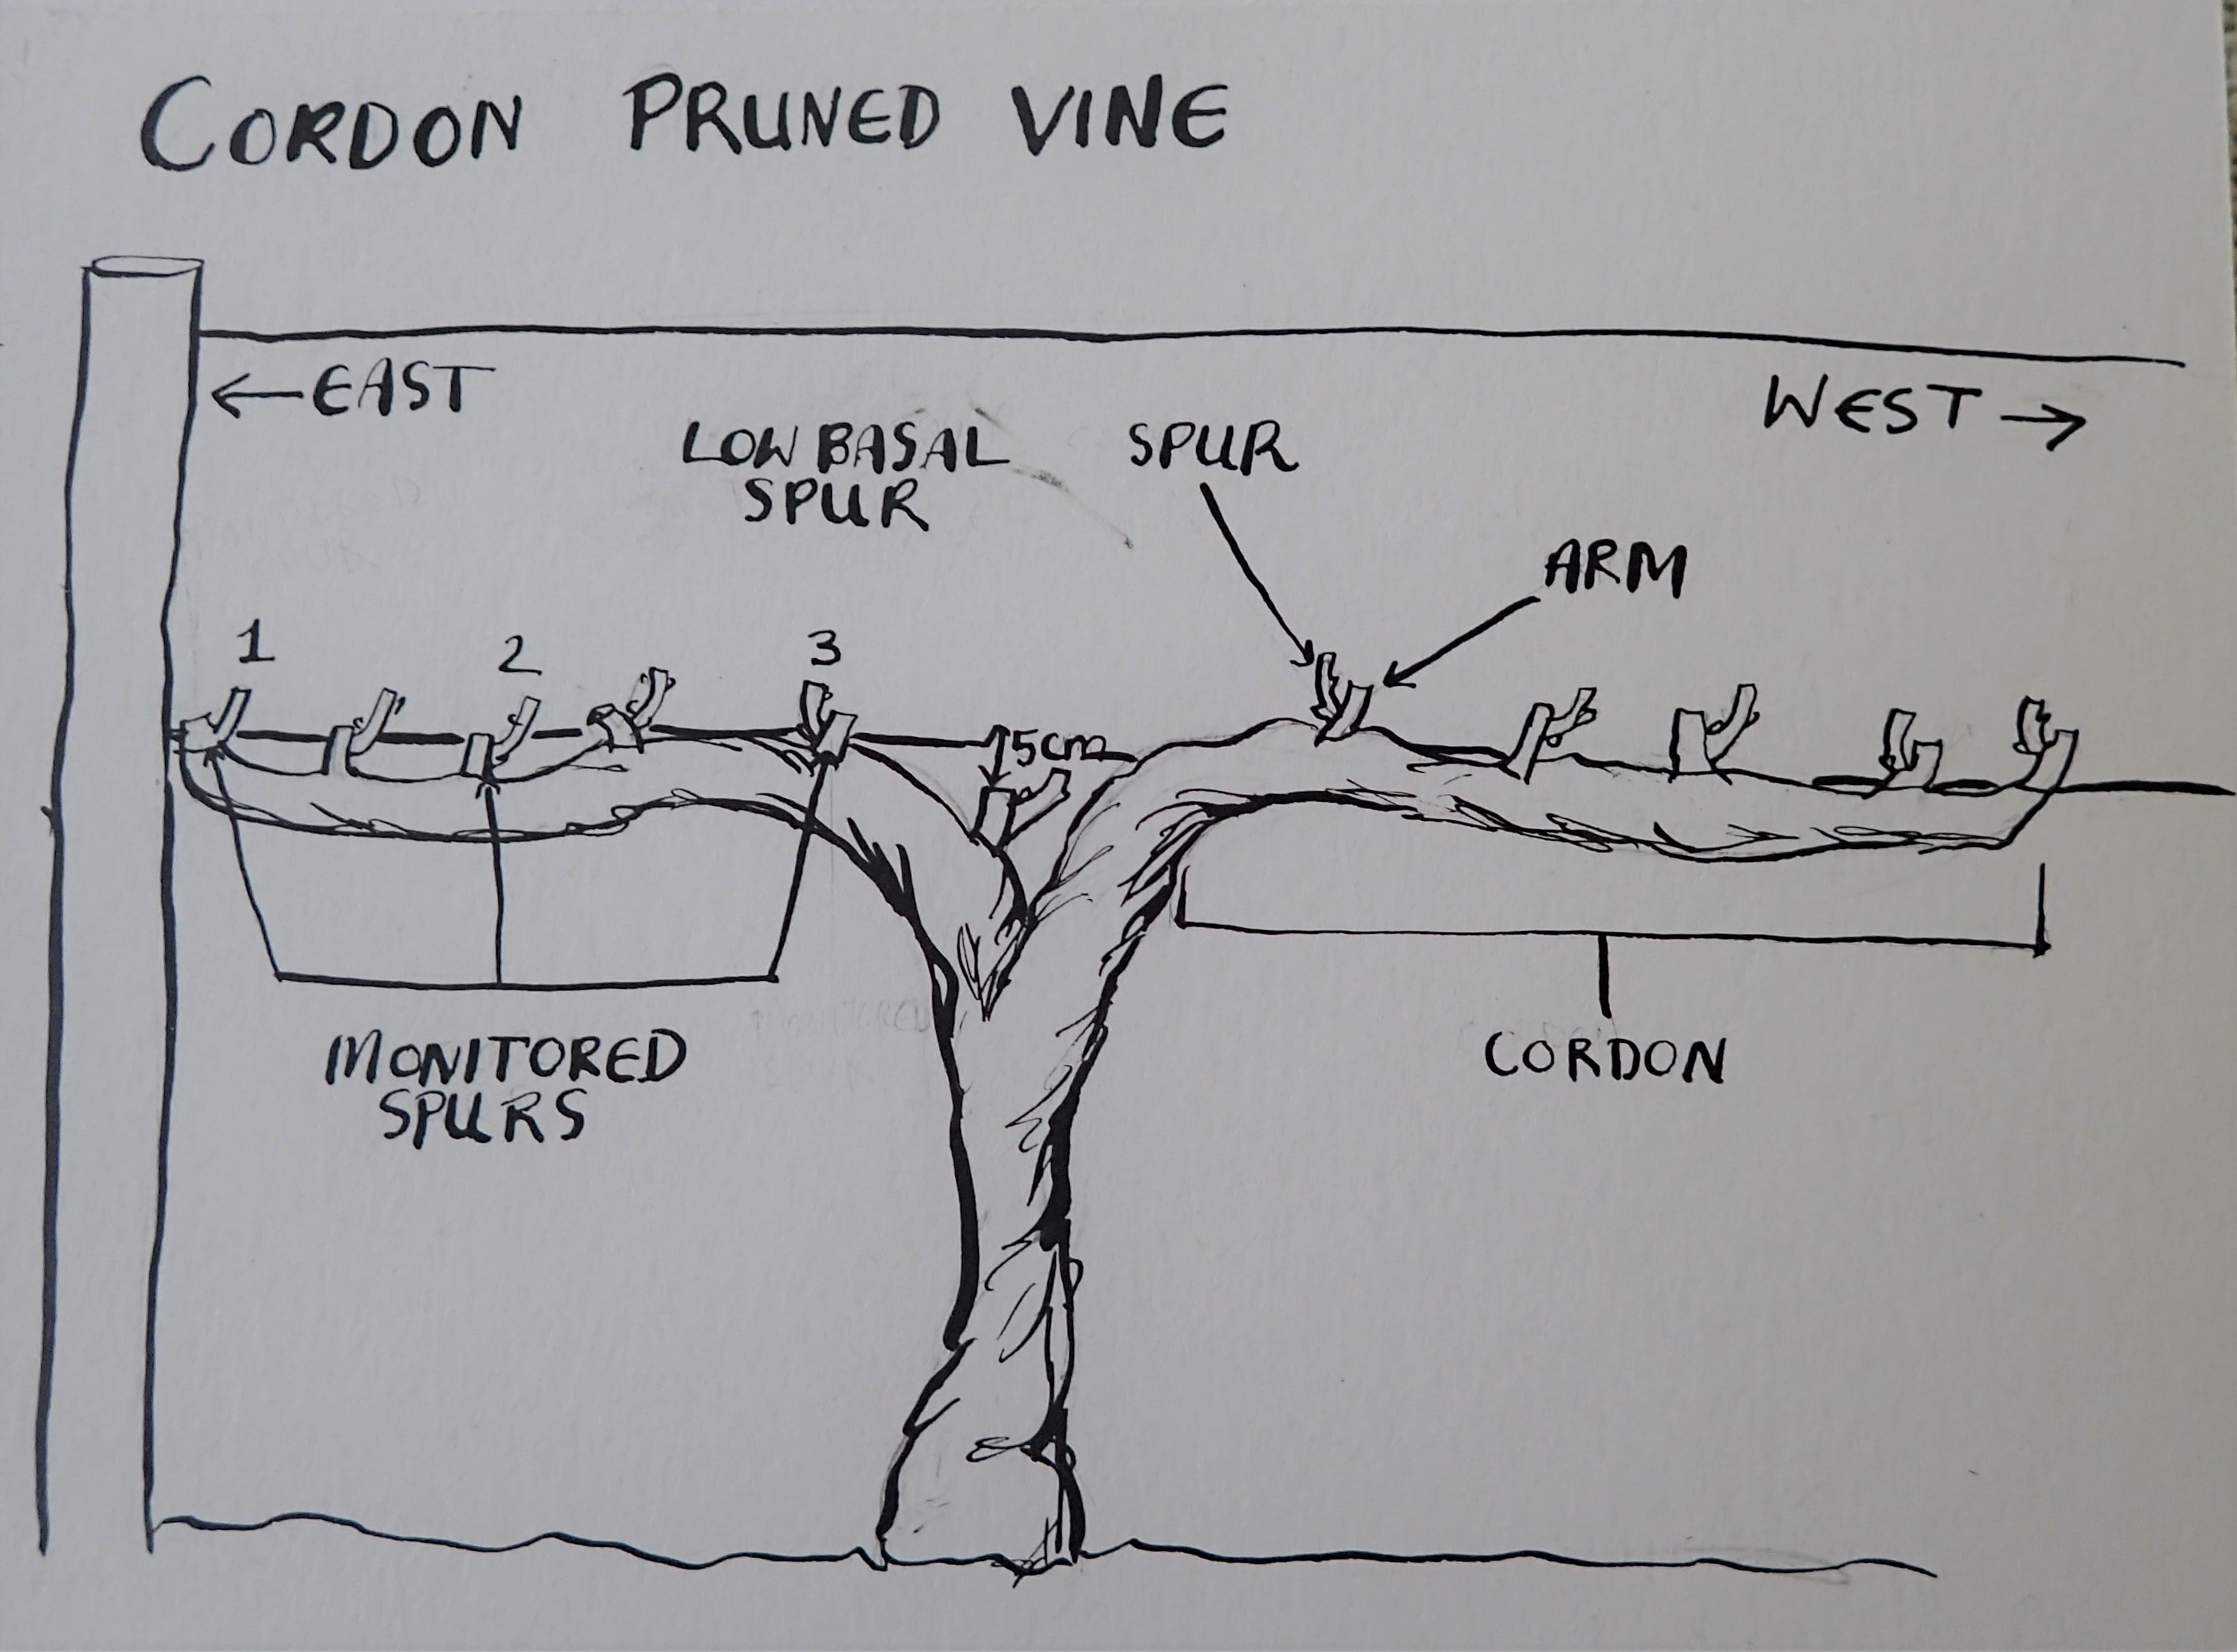
\includegraphics[width=\linewidth]{CordonPruned.jpg}
  \caption{A diagram of a cordon pruned vine, showing which spurs we would monitor. Any spur that's base was more than 5cm below the wire the cordon was trained on was not sampled. The buds in this diagram are incorrectly numbered.}
  \label{fig:CordonPruned}
\end{figure}

\begin{figure}
  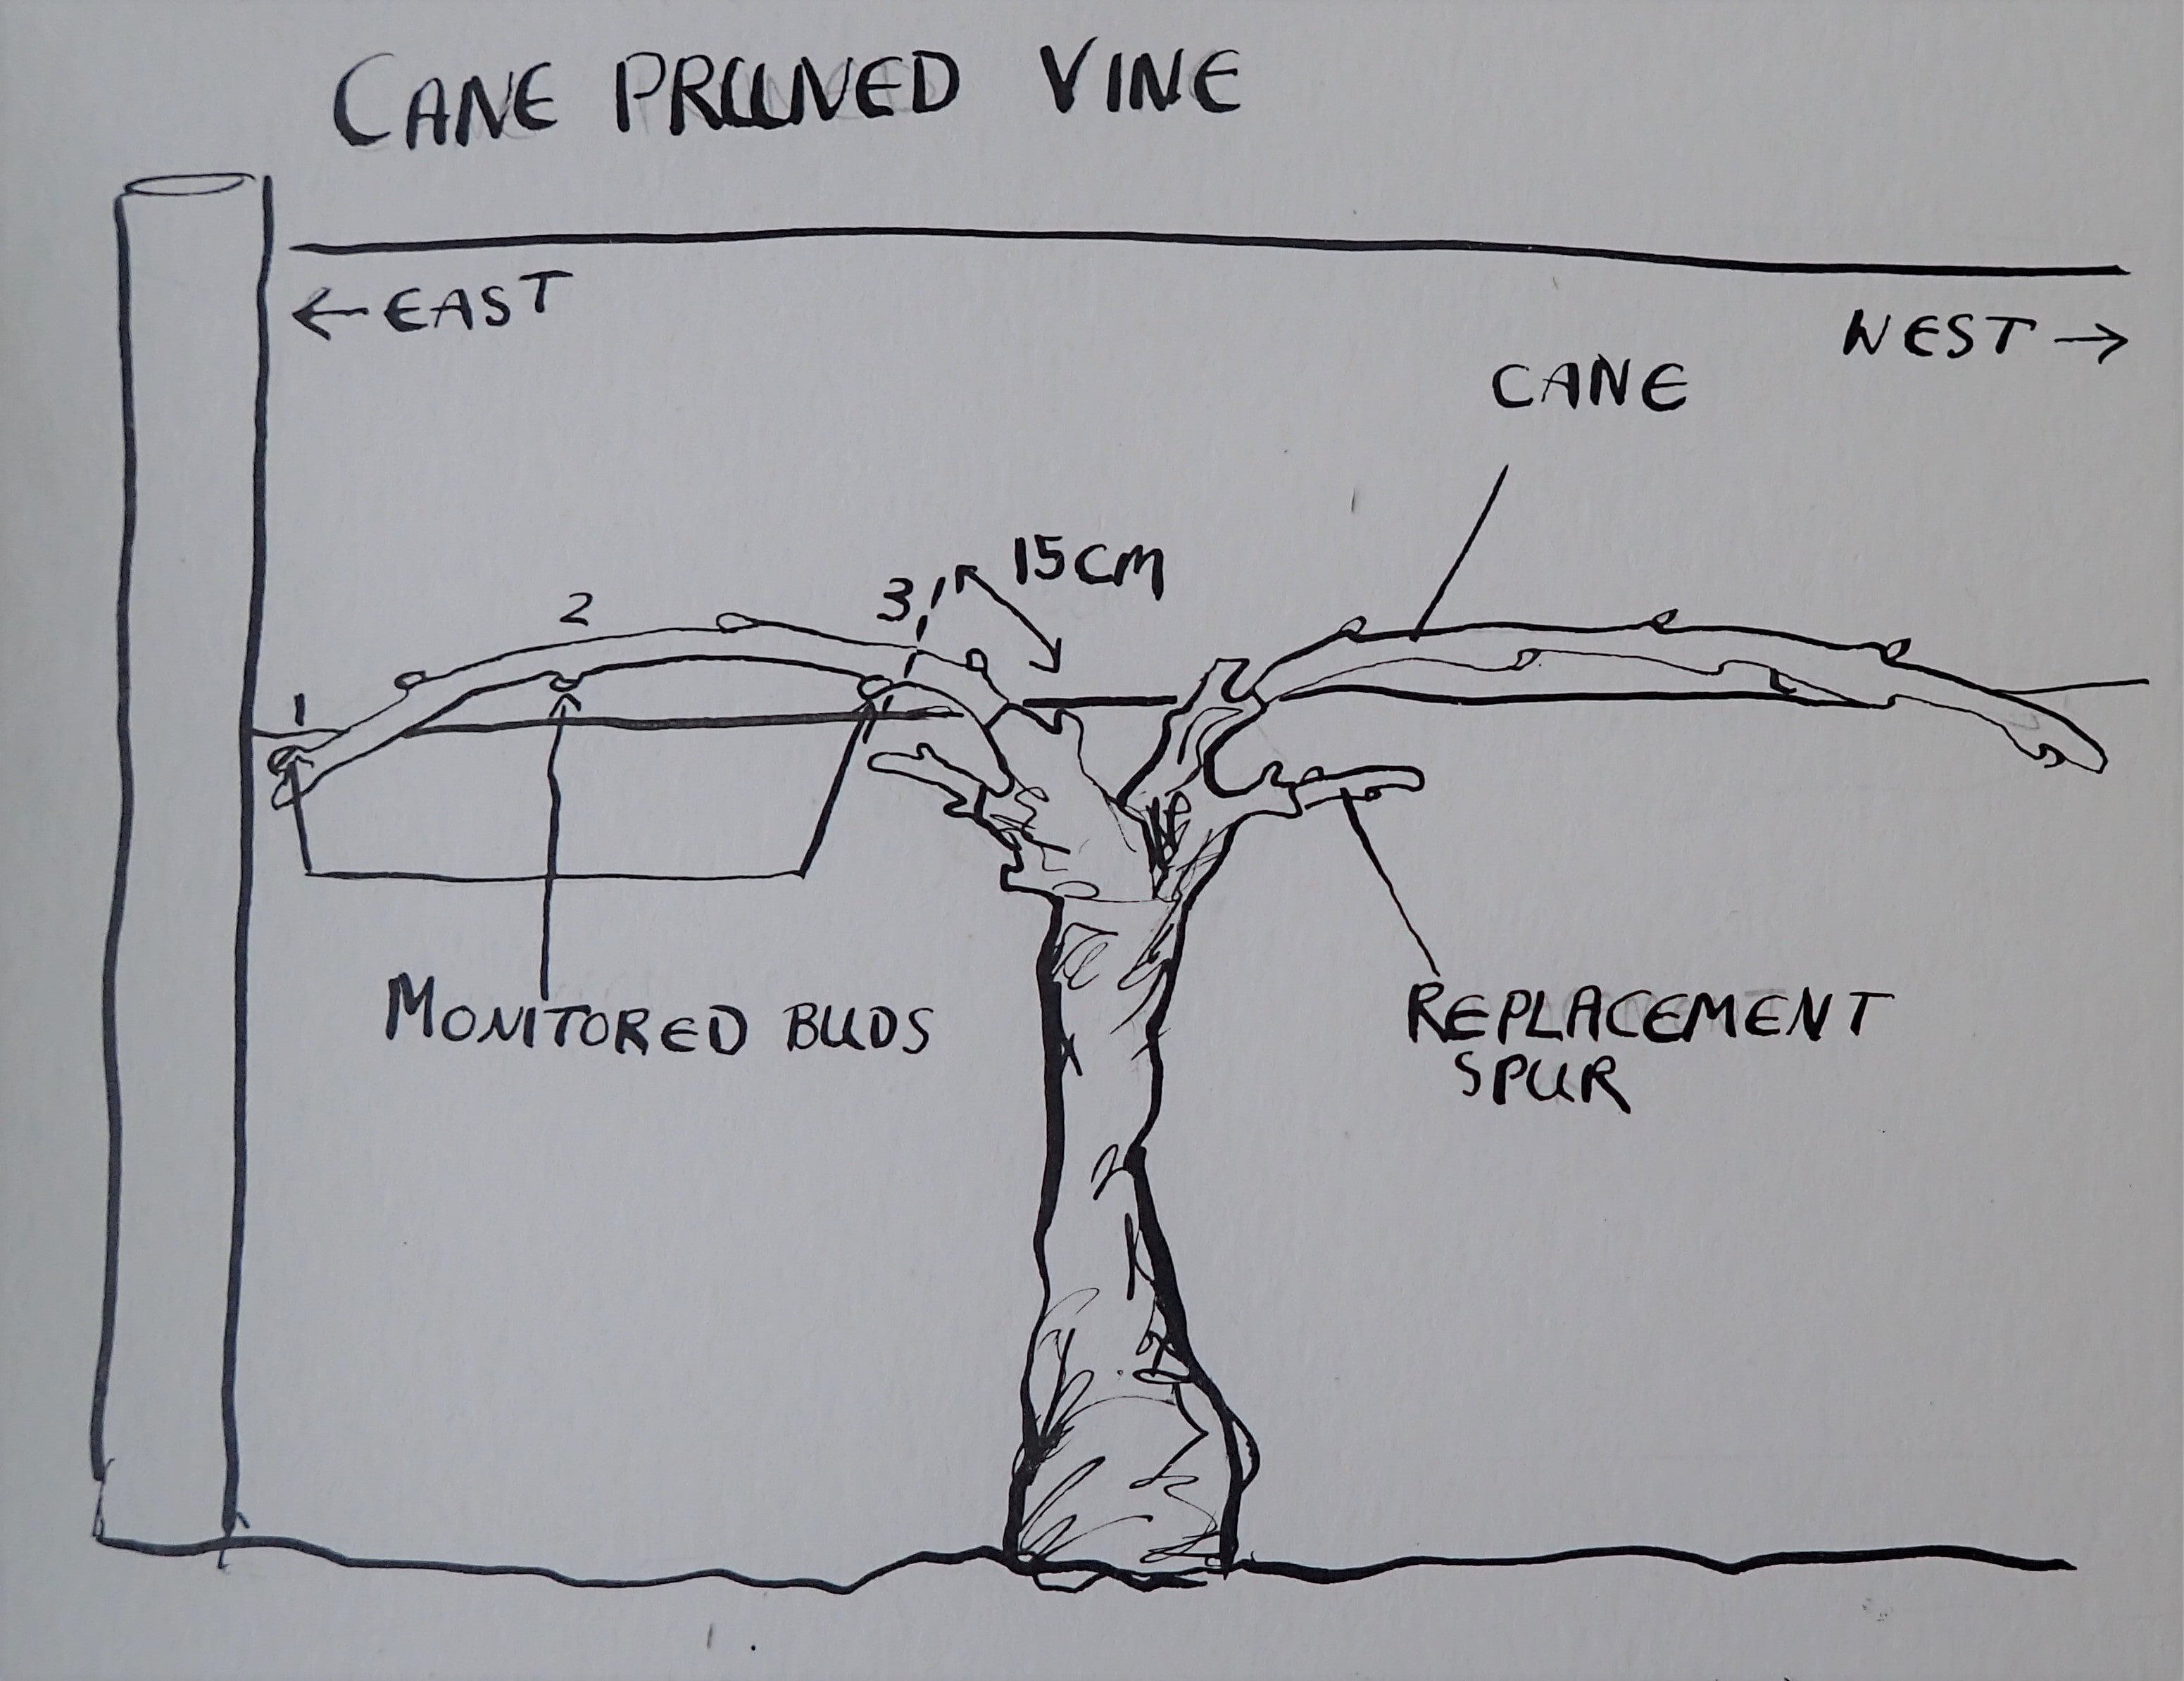
\includegraphics[width=\linewidth]{CanePruned.jpg}
  \caption{A diagram of a cane pruned vine, with the buds we would monitor. The bud numbering shown here is incorrect. Note that we do not sample buds too close to the head of the vine.}
  \label{fig:CanePruned}
\end{figure}

\begin{figure}
  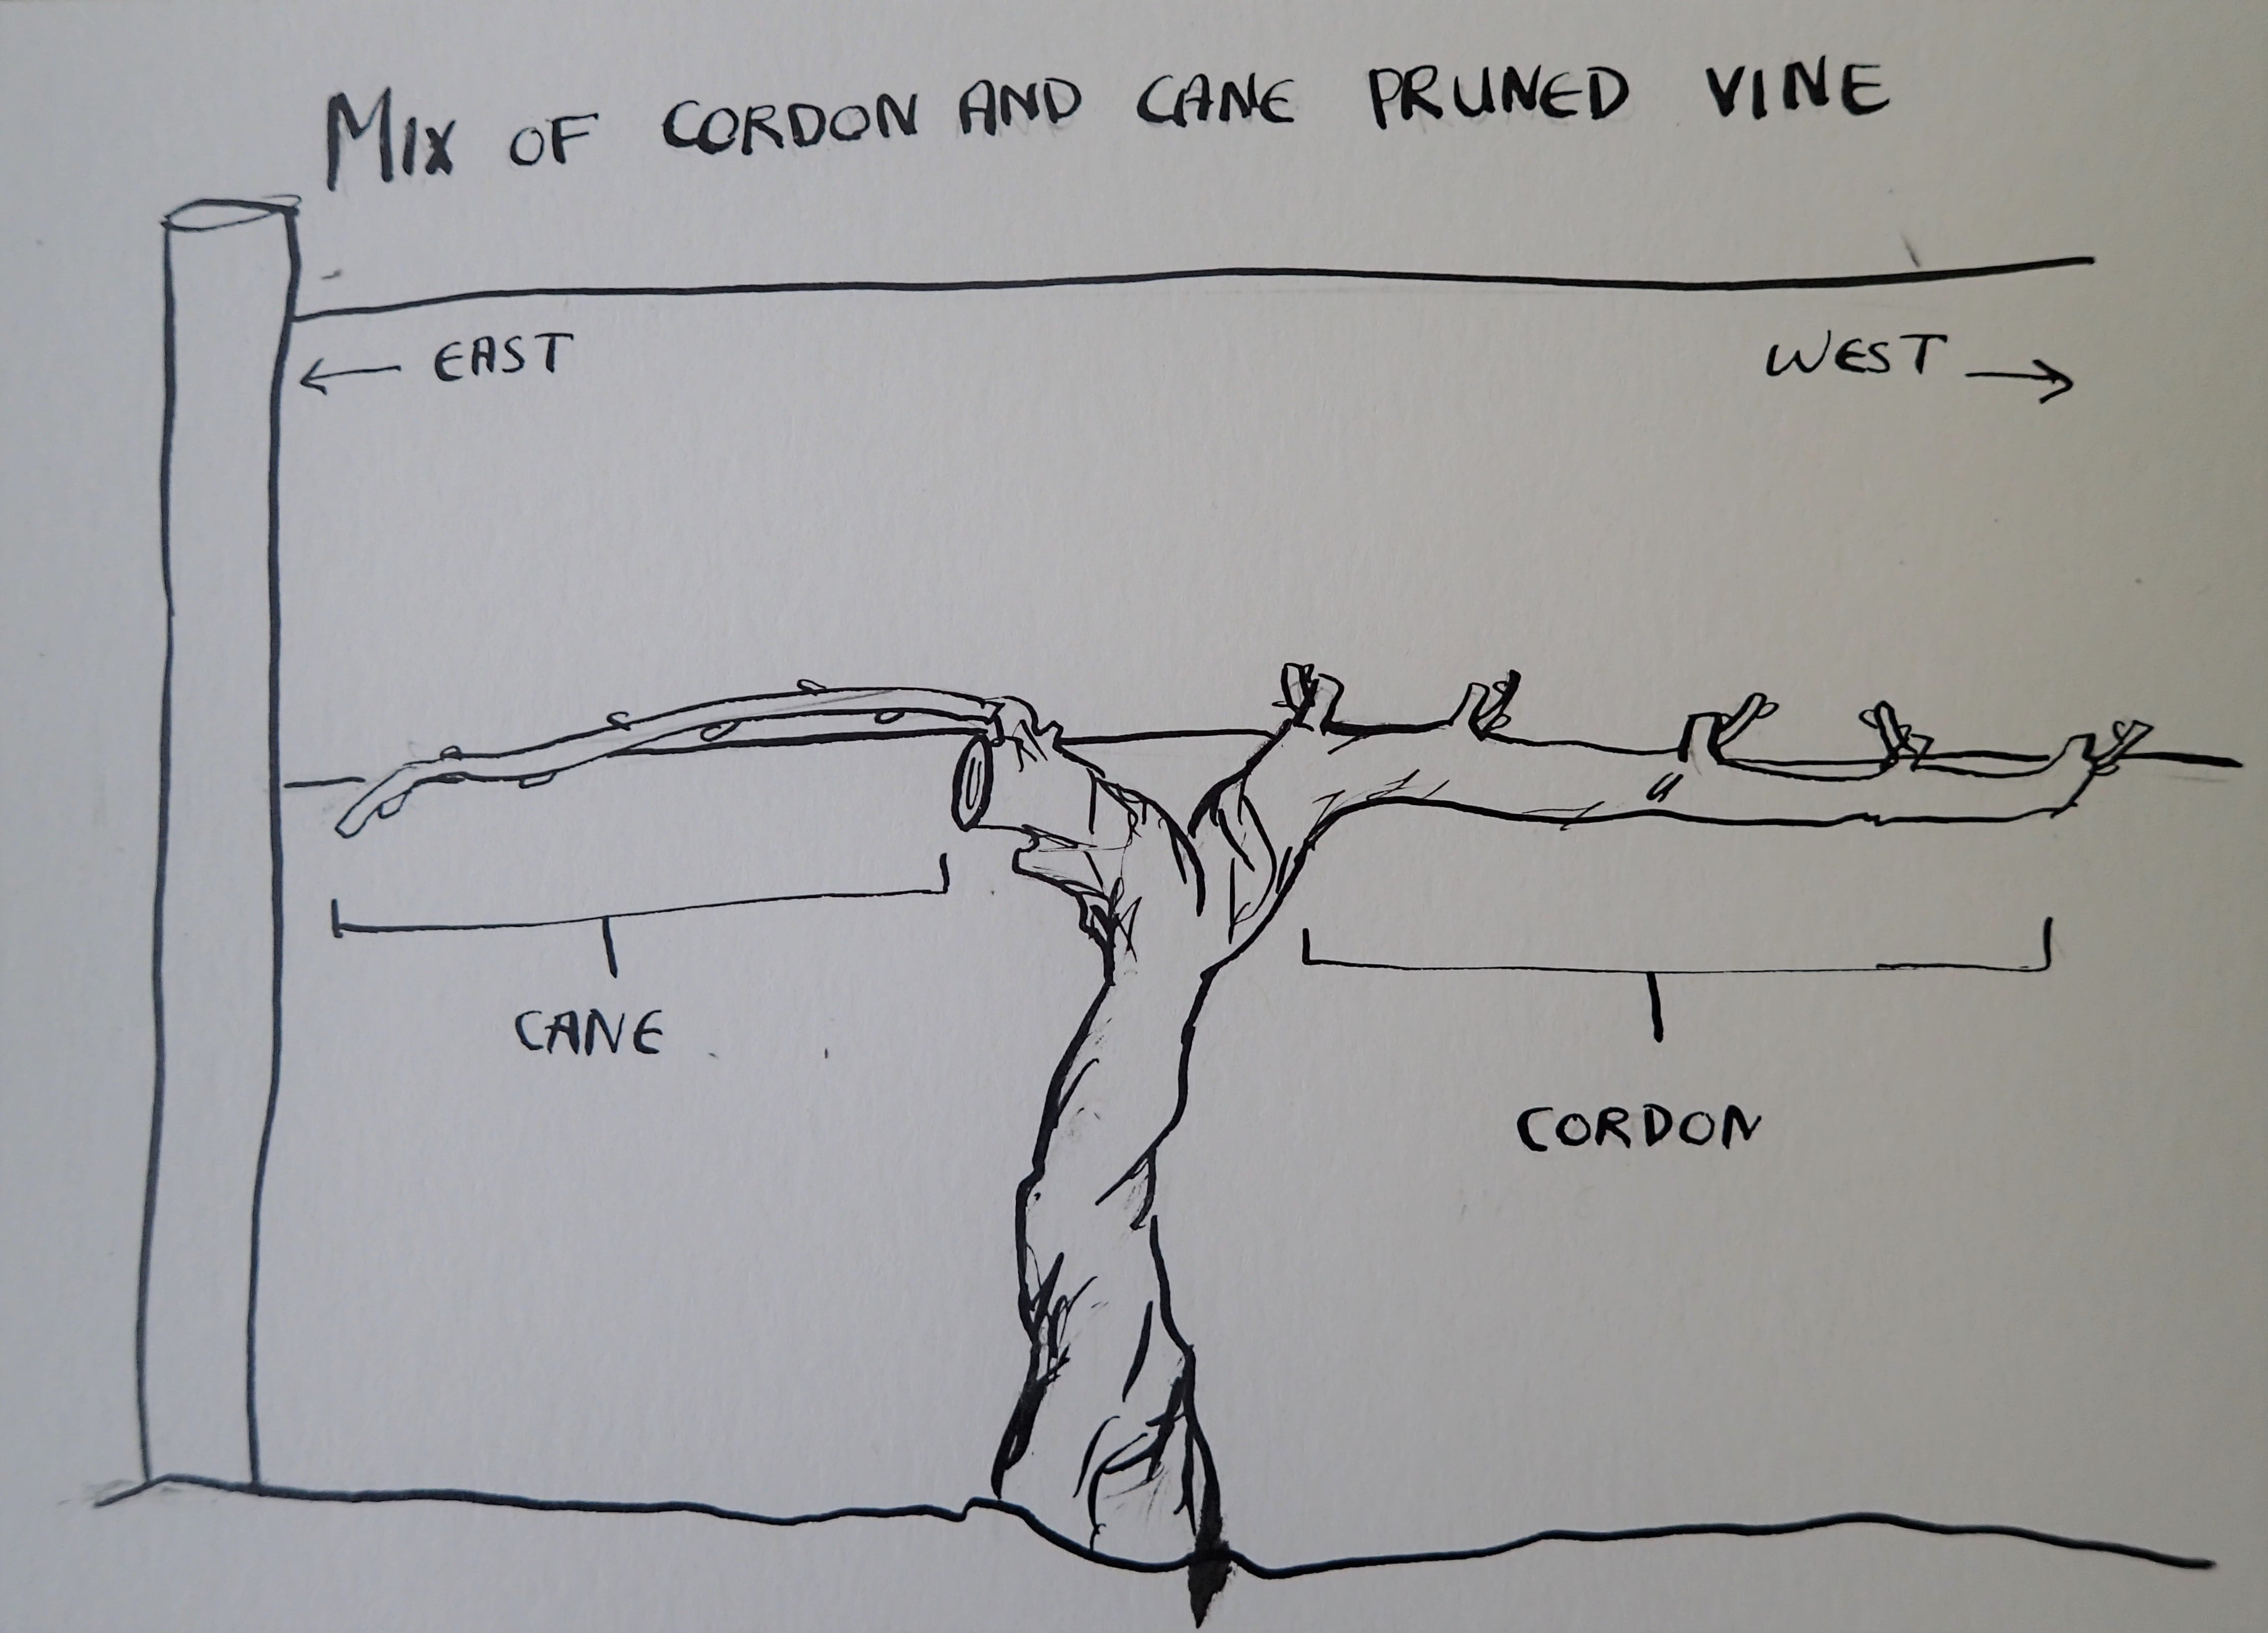
\includegraphics[width=\linewidth]{CaneCordonMix.jpg}
  \caption{When there is both a cordon and a cane, you we sample the cordon. The only time we would chose the cane rather than the cordon is if the cordon does not have enough spurs to sample.}
  \label{fig:CordonCane}
\end{figure}

\begin{figure}
  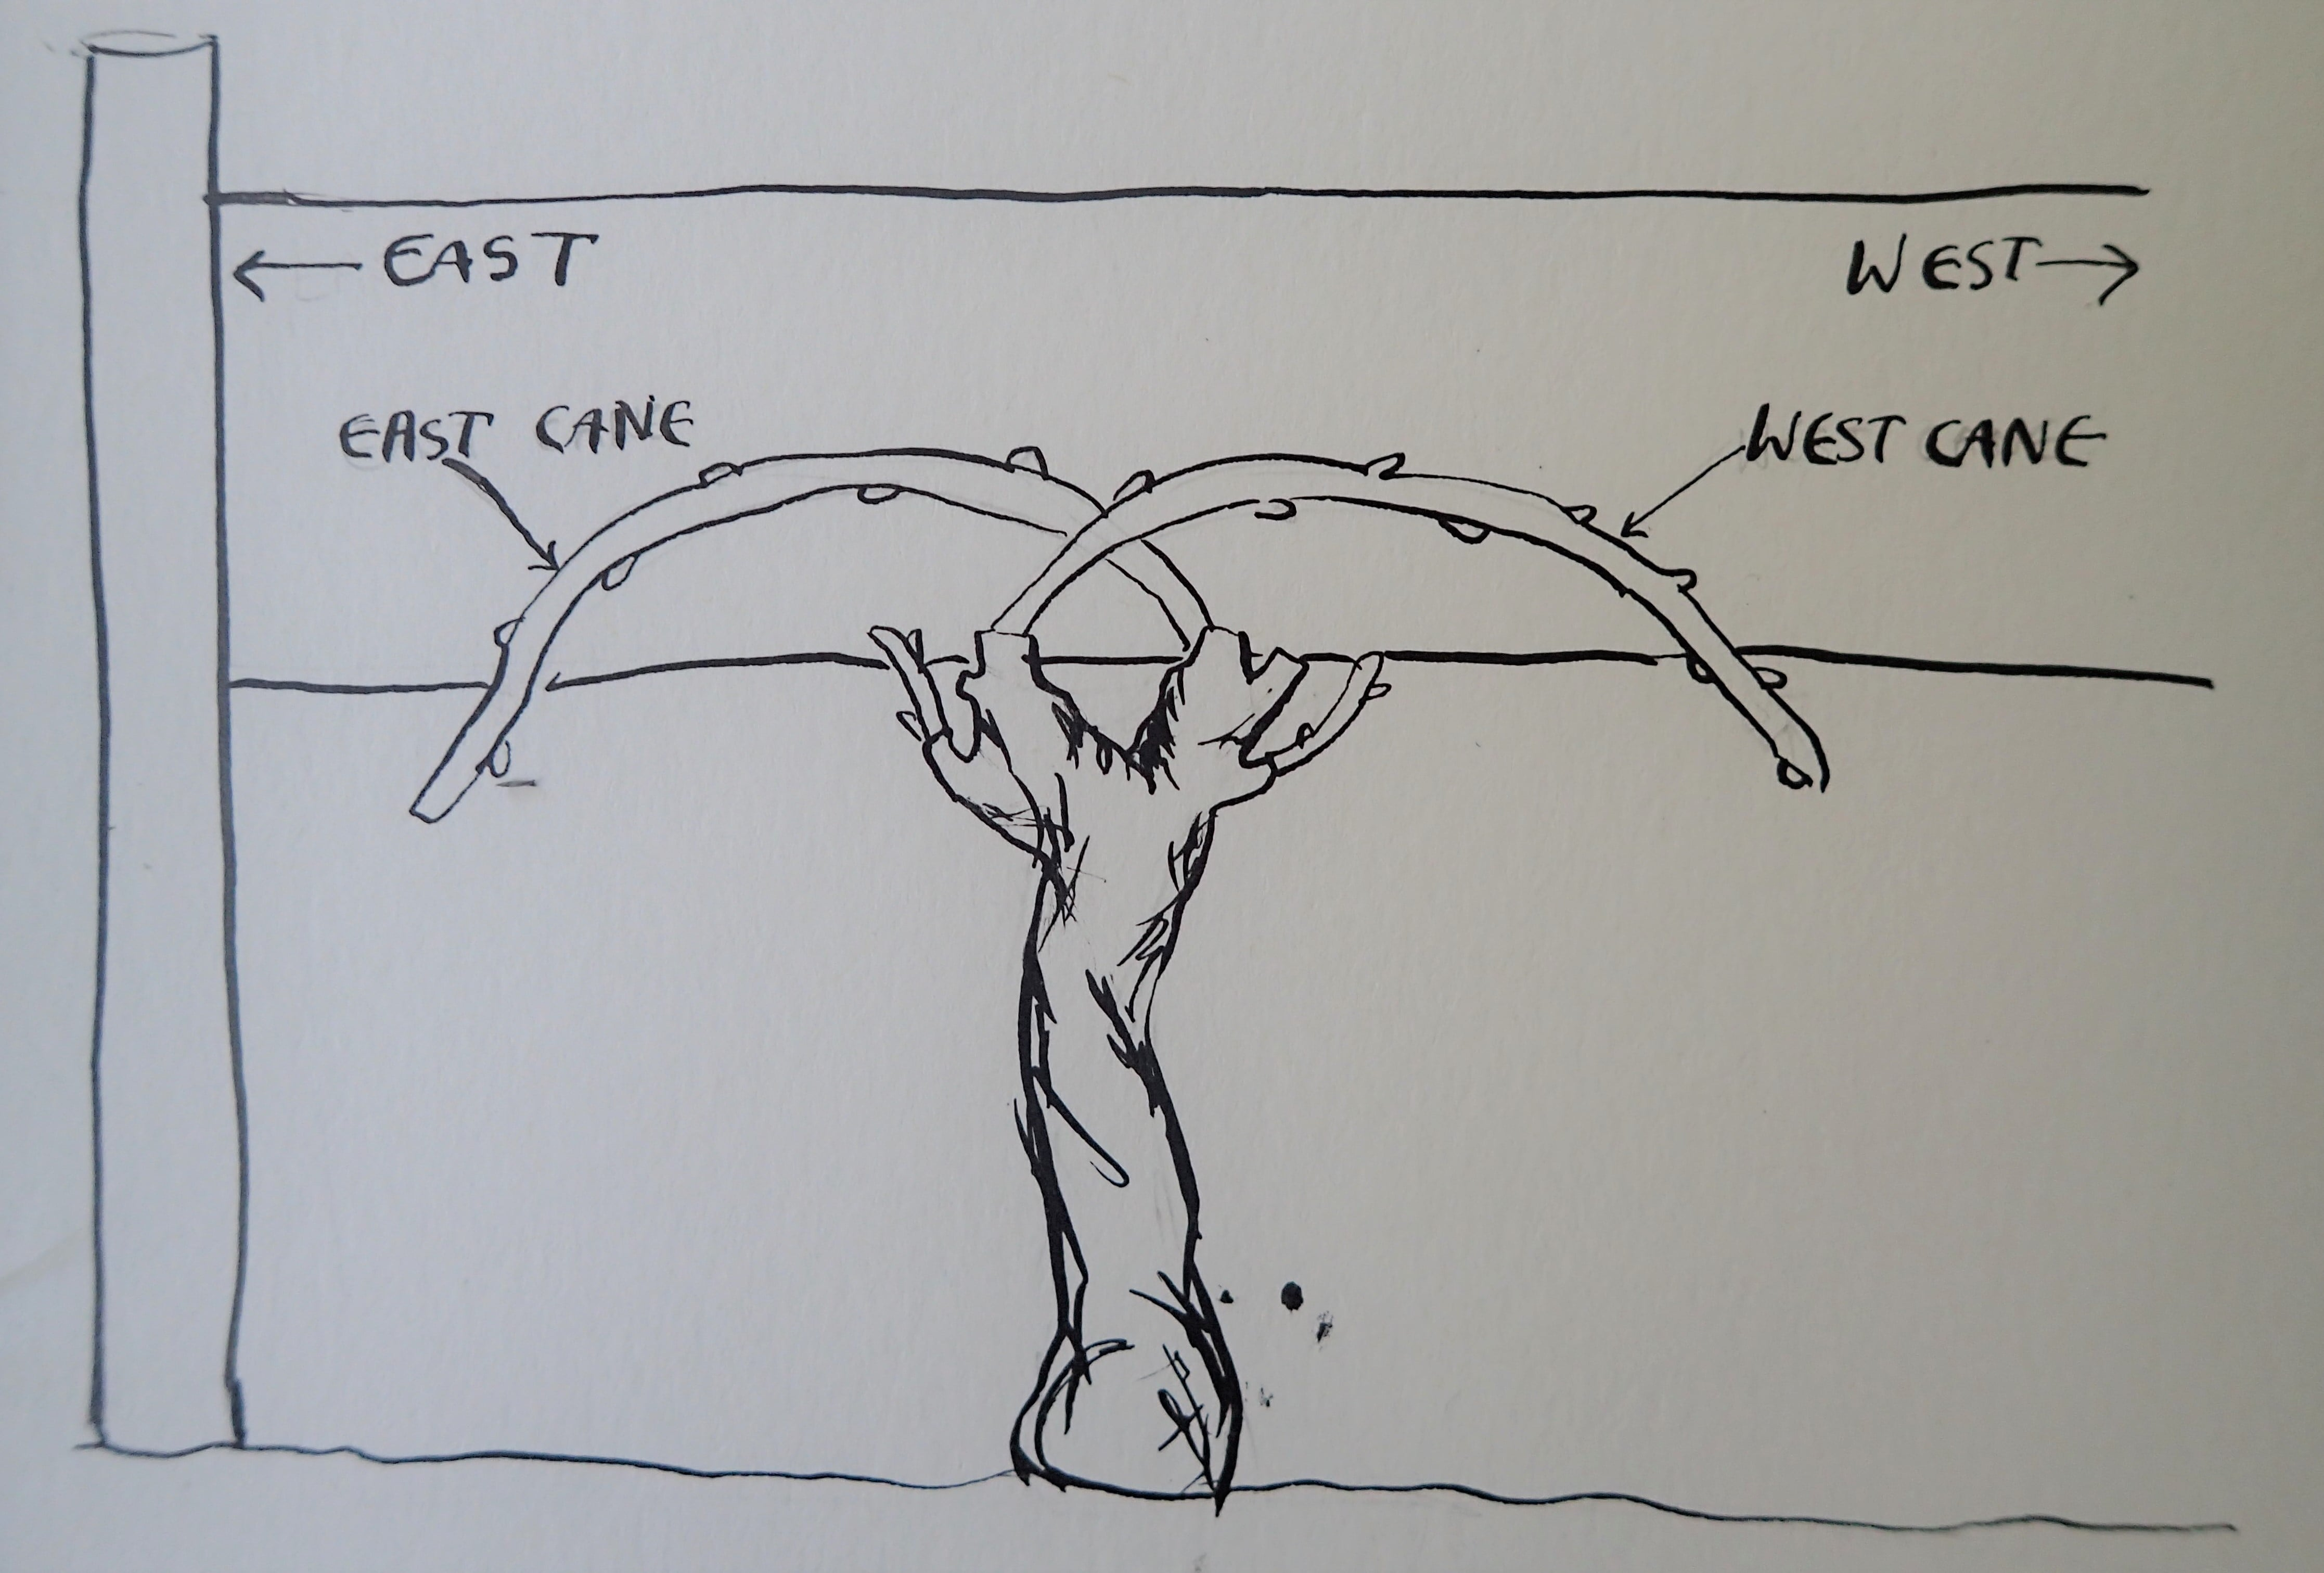
\includegraphics[width=\linewidth]{CaneCrossing.jpg}
  \caption{Sometimes the canes cross. If they do, we use the end of the cane to decide which side is east/west or north/south.}
  \label{fig:CaneCrossing}
\end{figure}

\begin{figure}
  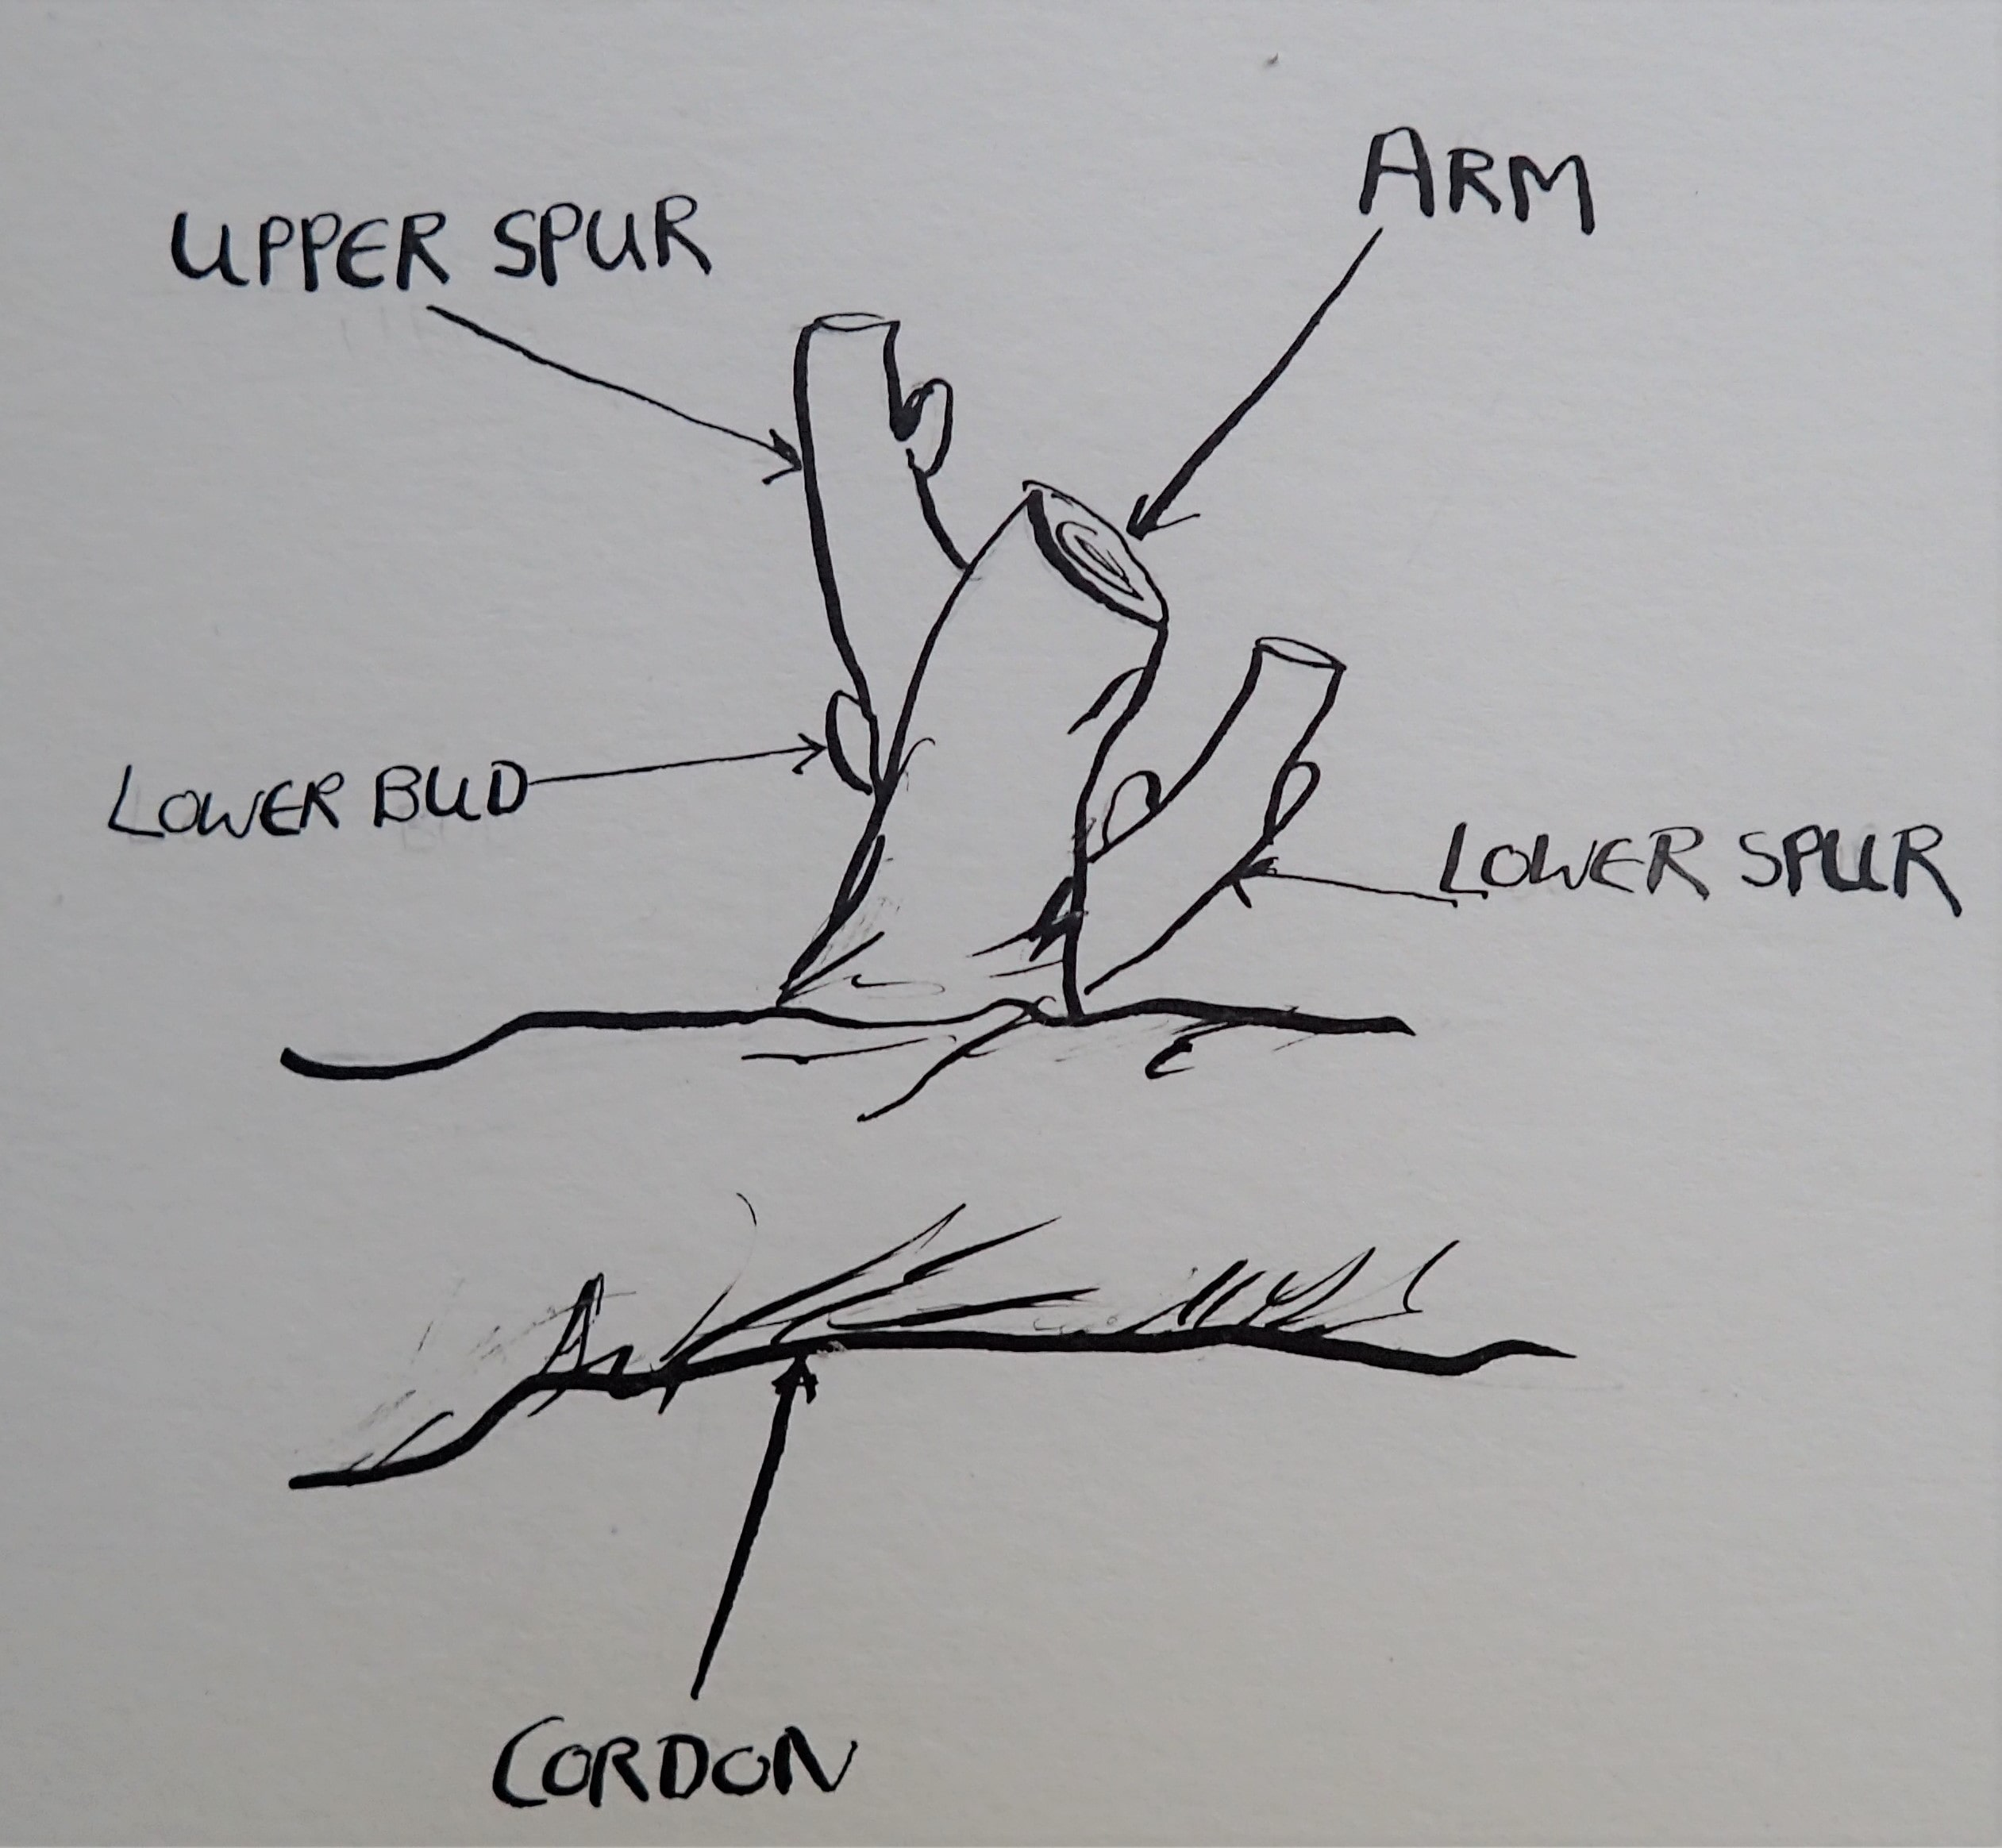
\includegraphics[width=\linewidth]{TwoSpurs.jpg}
  \caption{A diagram of an arm of a cordon that had two spurs on it. In this case we chose to focus on the lower bud of the higher of the two spurs for monitoring.}
  \label{fig:TwoSpurs}
\end{figure}



If plant was either cordon pruned (Figure \ref{fig:CordonPruned}) or cane pruned (Figure \ref{fig:CanePruned}, we flipped a coin to determine which side was flagged (heads = south or east, tails = north or west). If one side of the plant did not have enough buds, we chose the other side. If a plant had a cane and a cordon (Figure \ref{fig:CordonCane}, we flagged the cordon unless it did not have at least three spurs, then the cane was flagged. Occasionally, a cane would be trained back to the trunk in a loop or had come loose from the wire. (Figure \ref{fig:CaneCrossing}) In these cases, we flagged the other cane. If the cane started on one side but was trained to cross over and end on the other side, we used the direction of the end of the cane. 


\subsection{Cordon Buds}

We flagged the spur (or arm if it was present) on furthest from the trunk, a middle spur, and the first spur on the cordon with a base less than 5cm below the wire (Figure \ref{fig:CordonPruned}. Spurs more 5 or more centimeters below the wire were considered basal. If there was an even number of spurs, a coin flip determined which middle spur was chosen.

If there was more than one spur on an arm (Figure \ref{fig:TwoSpurs}) then we focused on the higher spur. We monitored the lowest bud on this spur. 

\subsection{Cane Buds}

We flagged the bud furthest from the trunk, the middle bud, and the first but that was farther than 15 centimeters from the trunk \ref{fig:CanePruned}. If there was an even number of middle buds, a coin flip determined which bud was chosen. 

If there were two buds in the same place in a position that was flagged, we chose to monitor the bud that was more upright. If both buds were equally upright facing, we monitored the one in a southerly or easterly direction. 

\section{Numbering Buds}
For the first set of data collection, Mira and Faith used this system: numbered the buds on each cordon or cane from 1 to 3, and numbered them in ascending order from either the south or the east. This caused confusion in the field so we decided to change the numbering protocol.

For the Dark Horse monitoring protocol and future monitoring seasons to the following:
Number buds 1 to 3 with bud 1 being the bud closest to the trunk. 

\section{Monitoring}

\begin{figure}
  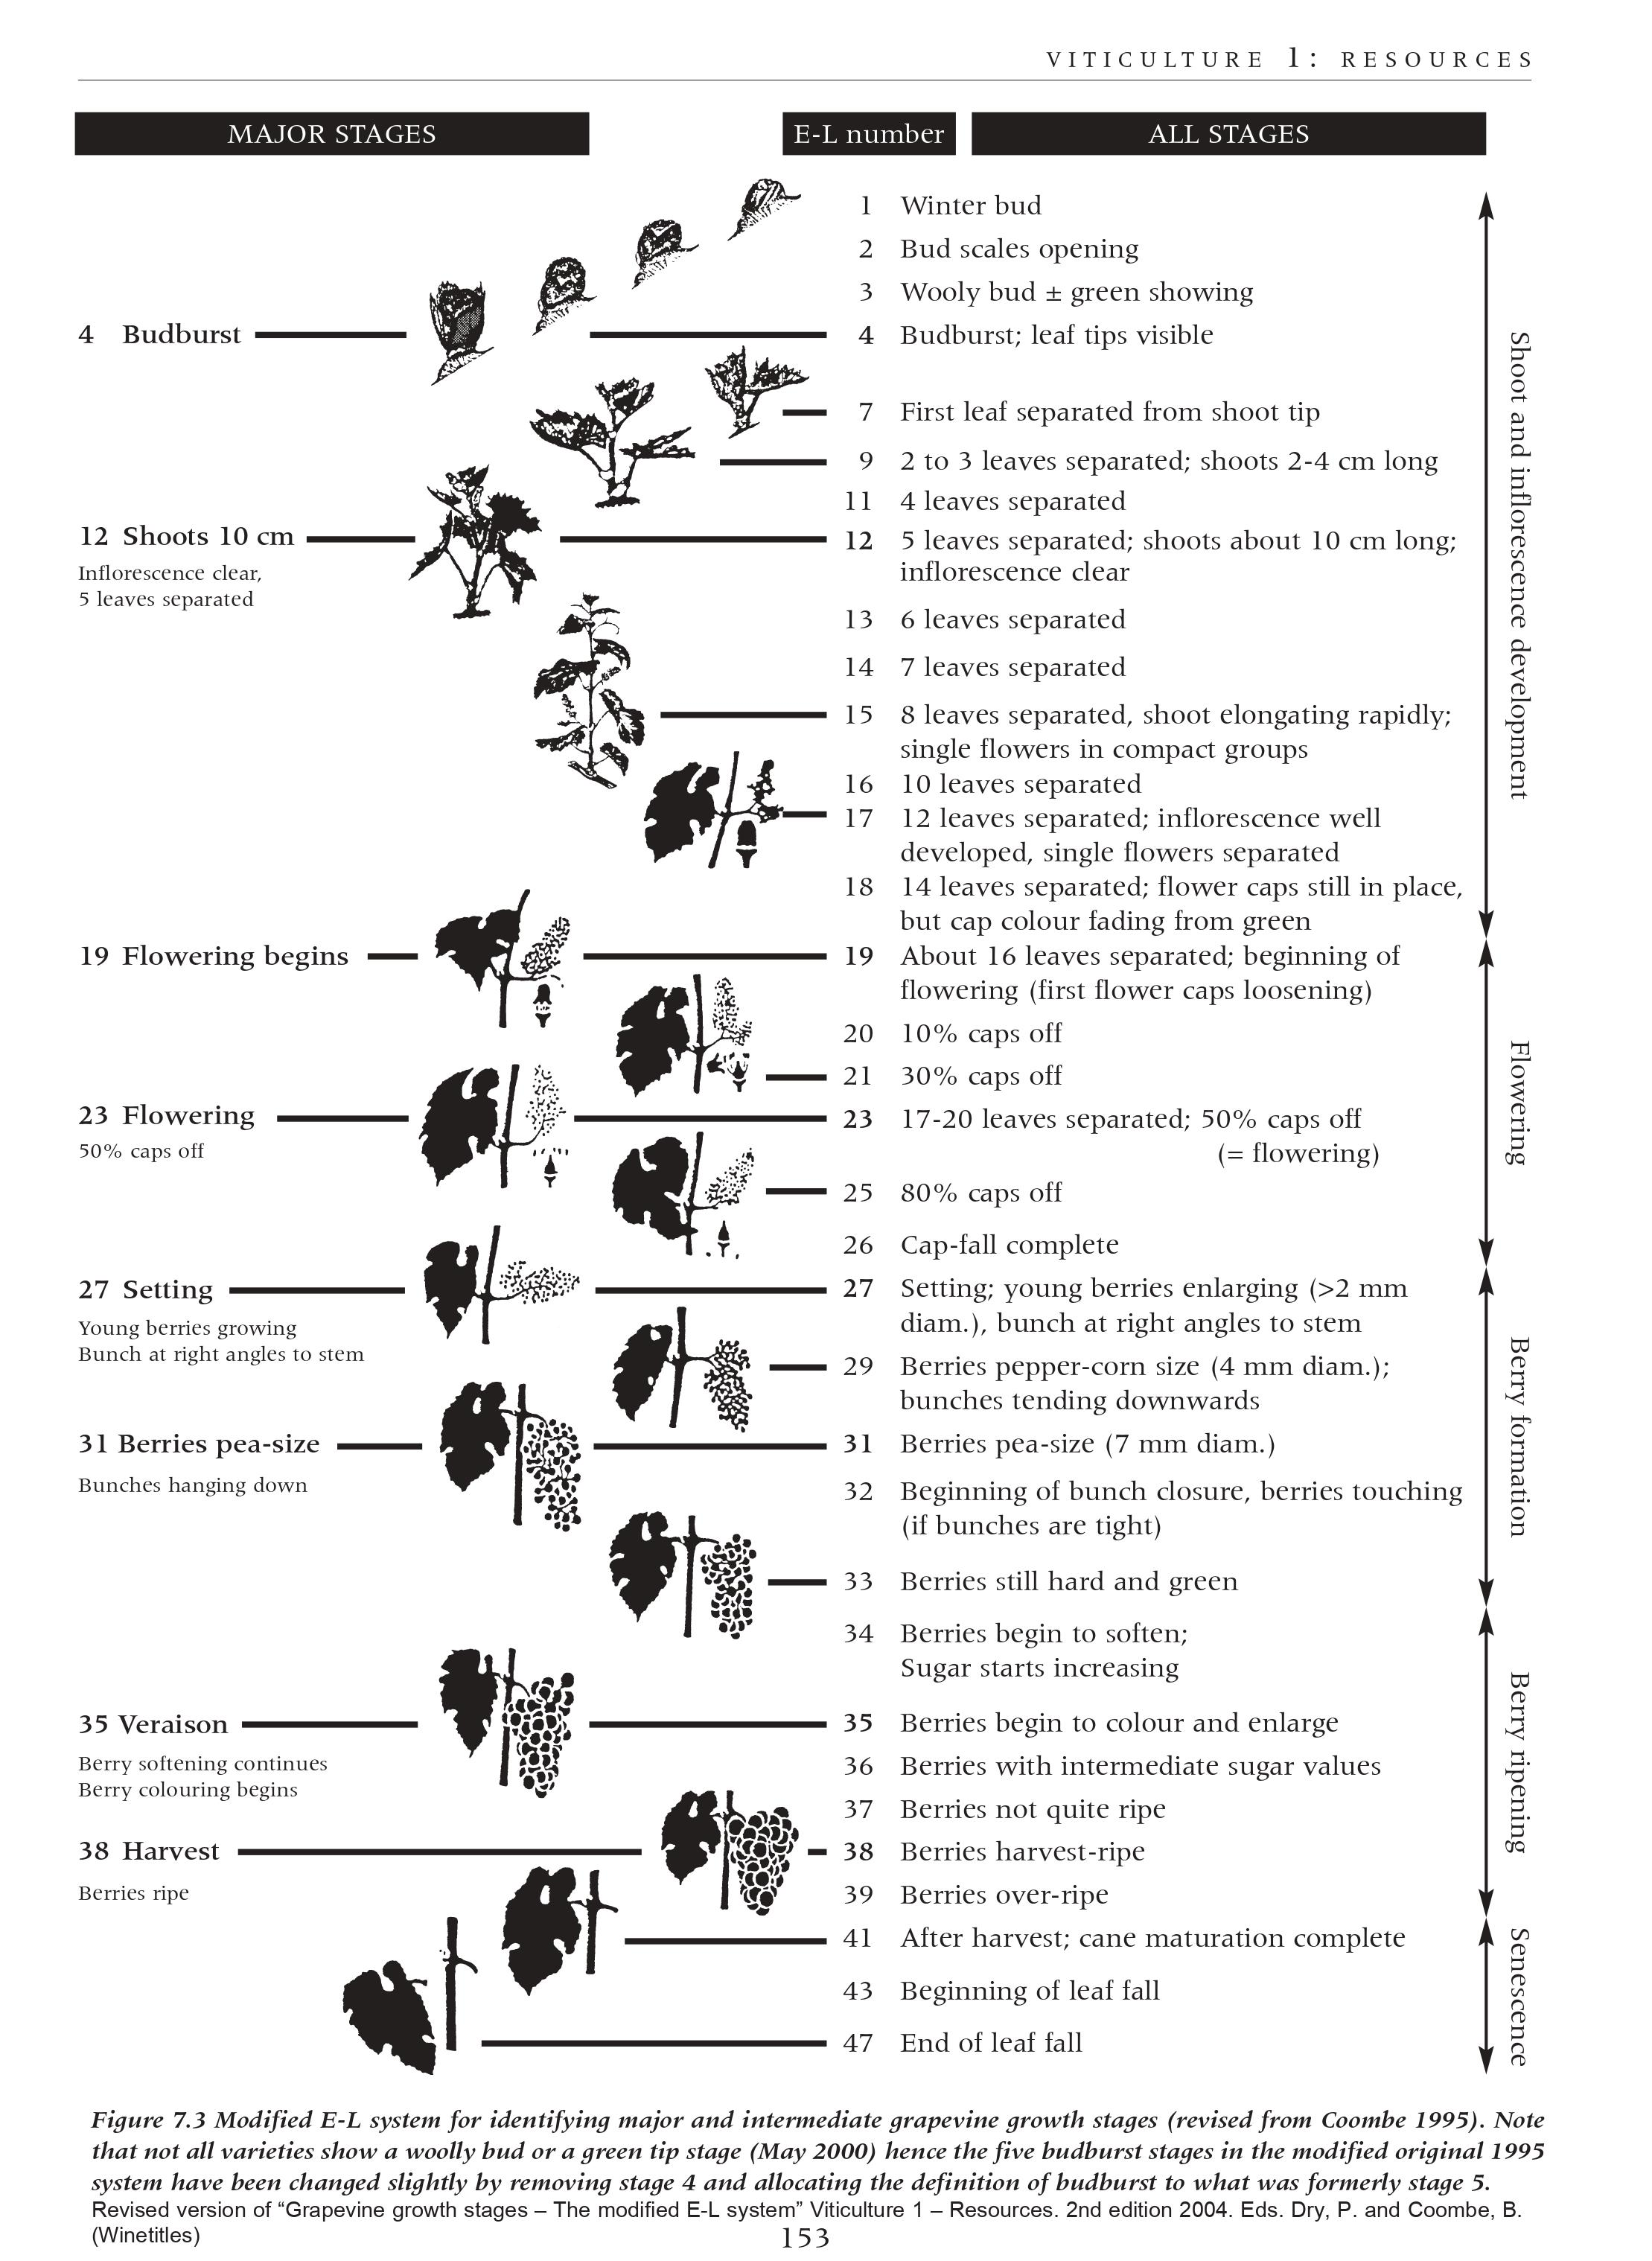
\includegraphics[width=\linewidth]{ELScale.jpg}
  \caption{ Modified Eichorn-Lorenz (EL) scale that our lab uses for monitoring phenology until flowering }
  \label{fig:ELScale}
\end{figure}

Our goal is to have standardized observations of phenological stages for analysis. There are four main widely observed stages for winegrapes: (1) budburst, (2) flowering, (3) veraison, and (4) ripening and harvest. For the first stage, budburst, we will use the stage numbers from the Modified Eichorn-Lorenz system (see Figure \ref{fig:ELScale}).For flowering and veraison, we will estimate the percent occurrence of the stage (proportion of berries on a selected cluster have gone through the stage of flowering or color change/softening, respectively). We will measure ripening quantitatively, using a refractometer to measure Brix.

\section{Sampling Frequency and Timing}

\begin{enumerate}
\item We will establish vines in March-April 2014 (labeling). 
\item We will then monitor four phenological stages: 
	\item Budburst (approx. March 15-Apr 10): Modification for 2016 onward: Until EL stage 9, record the EL stage of buds on three spurs. Once EL stage is at 9 you can stop recording until flowering starts (note that you may need to record higher than stage 9 at times in order to record whatever stage you see after 8, even if it is 12 or such if you have not yet recorded stage 9, more on this below).
	\item Bloom (approx. May 1-30)
	\item Veraison (approx. July 15-Aug 15)
	\item Ripening (Brix - approx Aug 15-Sept 30)
\item We estimate that observing pheno stages for each vine (budburst, bloom, and veraison) will take approximately 90s per vine. 
90 sec per vine x 256 vines at RMI variety display block = 6-7 person-hours to sample RMI
\item Once at least 5\% of the phenological stage (i.e., 5\% bloom) is seen, go out to the field until stage is complete for all varieties being monitored. 
\item During peak sampling, we will aim for techs to make pheno observations every 3 days (2x/week). 
\item Following the end of one pheno stage, techs will do a weekly vineyard walk-through starting 2-3 weeks before the anticipated beginning of the next stage, to make sure to catch early varieties entering the next stage.
\end{enumerate}

For each vine:
\begin{enumerate}
	\item Stand facing the vine. Double-check Plant ID (labeled on one of the flags), block, and row number before recording in correct place on data sheet that we will provide. You do not need to record information about the varieties on the datasheets.
	\item Bud numbers are not written on the flags but are numbered 1 to 3 with Bud 1 being the bud closest to the trunk.
	\item For pre-bloom, record the appropriate E-L stage of the shoot that was flagged, or the shoot closest to the flagging that matches our selection criteria laid out in the section above. Record its EL stage (number from “1”: still dormant, to “17”: twelve leaves separated- see \ref{fig:ELScale}) until EL stage 9. Once EL stage is at 9 you can stop recording until flowering starts (note that you may need to record higher than stage 9 at times in order to record whatever stage you see after 8, even if it is 12 or such if you have not yet recorded stage 9, more on this below).
	\item  For flowering (EL 23) and veraison (EL 35), look at each cluster (\#1, \#2, \#3) and estimate the percent (from 0-100\%) of berries on the sample cluster that have achieved that stage. 
	\item Take photos of representative illustrations for different varieties of target \% at stage (e.g., clusters at 5\%, 25\%, 50\%, 75\%, 95\% flowering) for different varieties. aim for 3-5 photos of each percentage taken across a diversity of varieties and across a couple different sampling dates, and make sure vine number and date are visible in photo for identification. {\bf Label the filename with the percent.}
	\item For ripening, our current plan is to send one of our team to collect berries so we can analyze Brix. We will aim to collect samples starting around 12-15 Brix until commercial harvest. 
	
\end{enumerate}

\section{Misc}
tape colors for QG are orange and blue, avoid flagging with these colors
Avoid orange and pink for Arterra - they seems to use of have most colors in their vineyards though
Ask vineyards at beginning of the season what color they prefer we use
Once at EL stage 7 or 9, flag bud itself?

\section{Contacting vineyards}

\end{document}

